The implementation of Cloud Simplify leverages a modern tech stack to achieve high throughput and security.

\subsection{Technology Stack}
The system is decomposed into several microservices, as summarized in Table \ref{tab:techstack}.

\begin{table}[h]
\centering
\caption{Technology Stack Decomposition}
\label{tab:techstack}
\begin{tabular}{|l|l|l|}
\hline
\textbf{Component} & \textbf{Technology} & \textbf{Description} \\ \hline
Frontend & React, Vite, CSS & Responsive Dashboard \\ \hline
Backend API & FastAPI (Python 3.x) & Asynchronous Web Services \\ \hline
Db & PostgreSQL & Persistent Storage \\ \hline
Orch. Engine & Celery + Redis & Task Queue \& Broker \\ \hline
Cloud Engine & Terraform & Multi-provider IaC Service \\ \hline
Container & Docker & Service Isolation \\ \hline
\end{tabular}
\end{table}

\subsection{Core workflows}

\subsubsection{Authentication Flow}
Security begins with a standards-compliant JWT authentication mechanism. Figure \ref{fig:auth_flow} illustrates the interaction between the user and the system.

\begin{figure}[h]
\centering
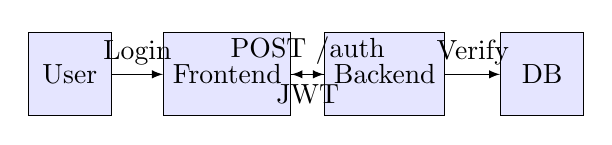
\begin{tikzpicture}[node distance=2cm, auto]
    \tikzstyle{actor} = [rectangle, draw, fill=blue!10, minimum width=3em, minimum height=3em]
    \tikzstyle{line} = [draw, -latex]

    \node [actor] (user) {User};
    \node [actor, right of=user] (front) {Frontend};
    \node [actor, right of=front] (back) {Backend};
    \node [actor, right of=back] (db) {DB};

    \draw [line] (user) -- node {Login} (front);
    \draw [line] (front) -- node {POST /auth} (back);
    \draw [line] (back) -- node {Verify} (db);
    \draw [line, dashed] (back) -- node {JWT} (front);
\end{tikzpicture}
\caption{Authentication Sequence}
\label{fig:auth_flow}
\end{figure}

\subsubsection{Provisioning Lifecycle}
The lifecycle of a cloud resource—from user interaction to final deployment—is managed through an event-driven sequence. As shown in Figure \ref{fig:lifecycle}, the FastAPI backend validates the request and offloads the intensive Terraform execution to a Celery worker via Redis.

\begin{figure}[h]
\centering
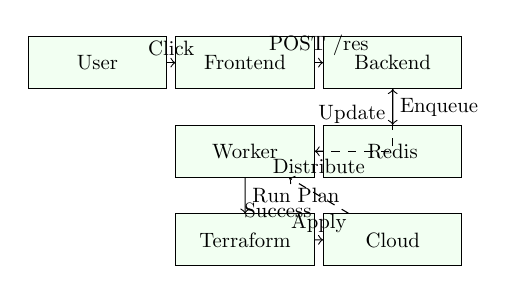
\begin{tikzpicture}[node distance=1.5cm, auto, scale=0.75, every node/.style={scale=0.75}]
    \tikzstyle{comp} = [rectangle, draw, fill=green!5, text width=6em, text centered, minimum height=2.5em]
    \node [comp] (u) {User};
    \node [comp, right of=u, xshift=1cm] (f) {Frontend};
    \node [comp, right of=f, xshift=1cm] (b) {Backend};
    \node [comp, below of=b] (r) {Redis};
    \node [comp, left of=r, xshift=-1cm] (w) {Worker};
    \node [comp, below of=w] (t) {Terraform};
    \node [comp, right of=t, xshift=1cm] (c) {Cloud};

    \draw [->] (u) -- node {Click} (f);
    \draw [->] (f) -- node {POST /res} (b);
    \draw [->] (b) -- node {Enqueue} (r);
    \draw [->] (r) -- node {Distribute} (w);
    \draw [->] (w) -- node {Run Plan} (t);
    \draw [->] (t) -- node {Apply} (c);
    \draw [->, dashed] (c) -- node {Success} (w);
    \draw [->, dashed] (w) -| node[pos=0.8] {Update} (b);
\end{tikzpicture}
\caption{The Provisioning Lifecycle Workflow}
\label{fig:lifecycle}
\end{figure}

\subsection{Code-Level Trace}
The internal execution path of a provisioning request is traced from the UI component to the Terraform module environment.

\begin{figure}[h]
\centering
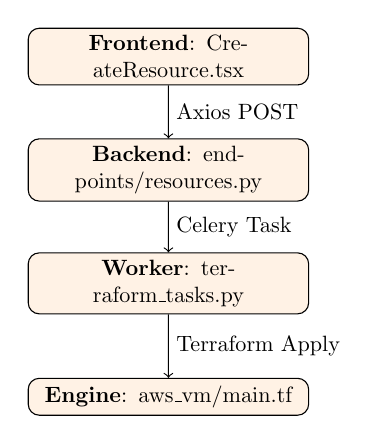
\begin{tikzpicture}[node distance=1.8cm, auto, scale=0.8, every node/.style={scale=0.8}]
    \tikzstyle{layer} = [rectangle, draw, fill=orange!10, text width=12em, text centered, rounded corners]
    
    \node [layer] (l1) {\textbf{Frontend}: CreateResource.tsx};
    \node [layer, below of=l1] (l2) {\textbf{Backend}: endpoints/resources.py};
    \node [layer, below of=l2] (l3) {\textbf{Worker}: terraform\_tasks.py};
    \node [layer, below of=l3] (l4) {\textbf{Engine}: aws\_vm/main.tf};

    \draw [->] (l1) -- node {Axios POST} (l2);
    \draw [->] (l2) -- node {Celery Task} (l3);
    \draw [->] (l3) -- node {Terraform Apply} (l4);
\end{tikzpicture}
\caption{Code Trace from UI to Cloud Provisioning}
\label{fig:code_trace}
\end{figure}

\subsection{Security and Encryption}
Security is implemented using a Zero-Trust architecture. 
\begin{itemize}
    \item \textbf{Identity Management}: JWT-based authentication with RS256 signing ensures that only authorized users can access the orchestration engine.
    \item \textbf{Data Security}: Cloud credentials (e.g., AWS Secret Keys) are encrypted using the \text{Cryptography} library in Python. The encryption keys are managed through environment-level secrets, isolated from the codebase.
    \item \textbf{Network Isolation}: When the Terraform engine runs, it executes in a transient worker environment with restricted network egress, ensuring that sensitive credentials are never leaked to external telemetry.
\end{itemize}

\subsection{Code Trace: Provisioning Logic}
The core provisioning logic resides in our \text{terraform\_tasks.py}. When an asynchronous task is received, the worker dynamically generates a workspace, symlinks the appropriate provider module, and executes the three-stage Terraform lifecycle: \textit{Init}, \textit{Plan}, and \textit{Apply}.
